\chapter{Discussion}\label{cha:discussion}

This chapter aims to discuss and critique the work that has been presented in this thesis. 

\section{Results}

In this section we discuss and draw conclusions from the experiments.

\subsection{Depth and ego motion}

From the experiments it appears that most options evaluated to alter the loss function does help to improve the results. Looking at experiment E7 where a maxed out SfMLearner architecture was trained and comparing it with experiment E11 where a very bare bones Monodepth2 architecture was trained we see that they have almost the same performance. This suggests that even though a good loss function is important, perhaps even more important is the underlying network architecture.

I am hesitant to draw any conclusions from experiment E9 and E10 where a model trained on Lyft performs better on Kitti than on the dataset it was trained on. This is so unexpected that I think it is more likely that the testing ground truth data is corrupt, but I have been unable to find any obvious problems with the data upon visual inspection.

Another surprise was the negligible effect of adding upscaling to the smaller depth maps. In the original paper it was claimed to be quite effective, but I was not able to come to the same conclusion.

It is quite clear from the results that the stationary pixel mask is more effective than the explainability mask. I also think there are further improvements that can be made here, as the stationary pixel mask is quite noisy.

Comparing experiment E3 and E4 we see that the edge aware depth smoothness loss does not help to improve the evaluation metrics. I still think it is valuable technique because the depth map looks sharper by visual inspection. Comparing experiment E4 and E5 we see that using SSIM in the photometric error and combining the per pixel loss across frames using the $\min$ function improves the metrics significantly.

\subsection{Keypoint detection}

The results from the keypoint prediction network was very satisfactory. One interesting property of the predicting network is that it rarely predicts keypoints at the edges of the image. I believe this might be because points near the edges in branch A are often outside of the image in branch A due to the homographic transformation. This means that predicting points near the edges would be penalized in the loss function during training because no correspondence would be found between points in branch A and B.

\subsection{Consensus maximization}

The results from the consensus maximization network is promising. But it seems to be sensitive to a few samples in the test set that throws it off completely thereby causing a large standard deviation in the mean homographic error (HE).

\section{Method}

This section aims to critique and discuss the method used to answer our research questions.

\subsection{Datasets}

Training the depth predicting network on Kitti and testing it on Lyft we can see that the depth maps produced (Figure \ref{fig:E14}) are quite acceptable. It is important for real world applications that the network is not over-fitted to its training dataset, but instead generalizes well to unseen data. Training and evaluating on two rather different car sequence dataset in this thesis was valuable in this regard, many papers only focus on getting the best benchmark on Kitti.

Using images from the Kitti dataset to train the keypoint prediction network gave the insight that the technique generalizes well to the domain of autonomous cars and navigation. In the original paper the network was trained on the HPatches\cite{hpatches} dataset. A drawback of using homographic transformation to train the keypoint network is that is it unclear if the keypoint network would generalize to images not related by a simple homographic transformation. In non planar scenes where the camera is moving in 3D, the feature points would instead be related by a fundamental matrix. To setup a system where unsupervised training could be performed on an image sequance such as the Kitti sequence dataset would be more complicated\cite{pose-sup}.

The consensus maximization network was trained on homographies because it was possible to implement it as a natural extension of the keypoint prediction pipeline. If the keypoint prediction training pipeline is altered to train on an image sequence, then the consensus maximization could predict a fundamental matrix instead of a homography, which also would be more appropriate to solve a structure from motion problem.

\subsection{Evaluation metrics}

Comparing the keypoint prediction network with the ORB detector in OpenCV was a compromise made because of the limited time and scope of this project. Perhaps it would have been more interesting to compare it against a more state of the art classical detector, or another neural network method of predicting keypoints. It was still valuable to see how the neural network method implemented in this thesis compared to ORB that is popular to use in practice.

The same could be said about the comparison between RANSAC and the consensus maximization network, perhaps a comparison other neural network techniques would also be desirable. But again the RANSAC algorithm in OpenCV is very popular in practice.

\section{Future work}

A very interesting path for future work would be to chain all networks together and train them at the same time. The joint training could possibly lead to better performance overall. Maybe the individual networks would have to be trained separately using the methods described in this thesis before chaining them together and then continue training using a joint loss function. The following is a suggestion for how the networks and their loss functions could be coupled together, illustrated in Figure \ref{fig:futurework}.

Two nearby images in the sequence dataset are fed into both keypoint net and depth net. The 2D positions from the keypoint net can be lifted to 3D by sampling the depth maps. The 3D points are fed into the consensus network configured to predict a rigid 3D transformation. The photometric error loss function is implemented as before (Figure \ref{fig:warp}). But instead of using a pose predicting network, the output transform from the consensus network is used instead.

Instead of calculating the point pair and correspondence matrices $\textbf{G}$ and $\textbf{C}$ using a known homography, we instead use the rigid 3D transformation to move the 3D points from $\textbf{I}_s$ and reproject them onto $\textbf{I}_t$. This uses the same method we use to reproject the image using the rigid transform and depth map, but this time it is done for sparse 3D points. The correspondances are calculated just as in section \ref{sec:keypointloss} but this time using the keypoints from $\textbf{I}_s$ and the reprojected points from $\textbf{I}_t$. The keypoint loss function would also be implemented as described in this thesis using the correspondences. Additionally a loss term could be added to encourage the keypoint score $\textbf{s}$ and the inlier prediction $\textbf{w}$ to be similar.

Having depth maps from two frames in the sequence, and point pairs that should represent the same points in the scene, we can also add a sparse depth consistency loss.

\begin{equation}
\mathcal{L}_{\mathrm{cons}}=\frac{
||\textbf{D}_t(\hat{\textbf{p}}_t) - \textbf{D}_s(\hat{\textbf{p}}_s)||
}{
\textbf{D}_t(\hat{\textbf{p}}_t) + \textbf{D}_s(\hat{\textbf{p}}_s)
}
\end{equation}

This sparse loss reduces scale drift of the depth maps across frames.

\begin{figure}[H]
	\centering
	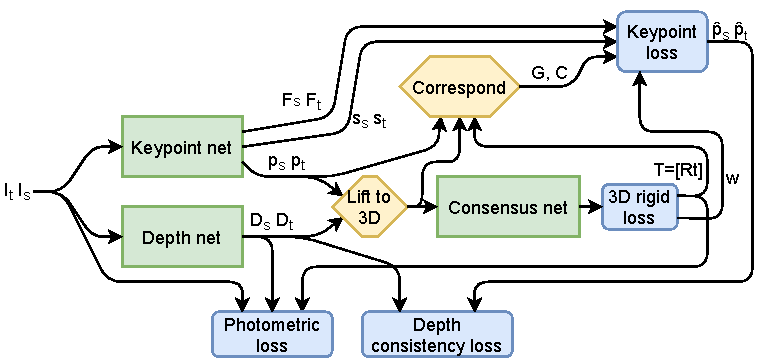
\includegraphics[width=0.8\textwidth]{future-work}
	\caption{A diagram with a suggestion of how the networks presented in this thesis could be chained together and trained using a joint loss function.}
	\label{fig:futurework}
\end{figure}

\section{The work in a wider context}

Self driving vehicles is a key area where neural network perception has a big impact. The adoption of autonomous vehicles could lead to more ride sharing alternatives, reducing the demand for owning a car, which in turn could reduce road congestion and oil consumption. \cite{transportation}

A common concern with autonomous technologies is the impact it could have on available job opportunities. Truck drivers are often brought up as a profession that will be especially hard hit. The advent of wide spread autonomous driving vehicles could also bring about many new professions not present today, the actual total outcome of available jobs is still an open debate.\cite{sociology}

TODO: MORE STUFFS!!!